\documentclass[8.01x]{subfiles}
\begin{document}

\chapter{Midterm 1}

\section{Problem 1: Derivatives and vectors}

``A point particle has a position vector $\vec{r}(t)$ as a function of time $t$, given by

\begin{equation}
\vec{r}(t) = (2-t^2)\hat{x} - 2t(t+4)\hat{y} + 10(t+2)\hat{z}
\end{equation}

where distances are in meters, and time $t$ is in seconds. Now, let $t = t_1 = 14$ s.

(a) What is the distance of the particle to the origin at time t1 ? (in meters)''

In other words, what is the magnitude of $\vec{r}(t)$ when we substitute $t = \SI{14}{s}$ into the equation:

\begin{align}
\vec{r}(t_1) &= (2-14^2)\hat{x} - 2\cdot14(14+4)\hat{y} + 10(14+2)\hat{z}\\
          &= -194\hat{x} - 504\hat{y} + 160 \hat{z}
\end{align}

The magnitude is found as $\sqrt{r_x^2 + r_y^2 + r_z^2}$, so

\begin{equation}
|\vec{r}(t_1)| = \sqrt{317252} \approx \SI{563.25}{m}
\end{equation}

``(b) What is the speed of the particle at at time $t_1$? (in m/s)''

We can differentiate the position equation with respect to $t$:

\begin{align}
\vec{r}(t) = (2-t^2)\hat{x} - (2t^2+8t)\hat{y} + (10t+20)\hat{z}\\
\frac{d}{dt} \vec{r}(t) = \vec{v}(t) = (-2t)\hat{x} - (4t+8)\hat{y} + (10)\hat{z}
\end{align}

We then again make the substitution for $t = \SI{14}{s}$, and then take the magnitude, and find 

\begin{align}
\vec{v}(t_1) = (-2 \cdot 14)\hat{x} - (4 \cdot 14 + 8)\hat{y} + (10)\hat{z}\\
|\vec{v}(t_1)| = \sqrt{(-28)^2 + (-64)^2 + 10^2} = \sqrt{4980} \approx \SI{70.57}{m/s}
\end{align}

``(c) What is the (smaller) angle between the velocity vector at time $t_1$ and the $\hat{z}$ axis? (in degrees)''

Hmm. I got this answer right on the exam, but when having a closer look, I noticed that my answer was actually off by 0.9\% (less than 1 degree, but read on).\\
Comparing my solution and the staff's, it's clear that my solution can give much, much greater errors for other components, so I got ``lucky'', getting it marked correct on my first try, despite an invalid method. Had $v_z$ been much larger, I would've gotten it wrong (though would have had a second try remaining). Anyway, long story short, I rewrote this answer to use a proper solution.

The staff's solution used the dot product -- I didn't think of that, clever. Let's try to calculate it that way.\\
We know that the dot product is $\vec{a} \cdot \vec{b} = |\vec{a}| |\vec{b}| \cos \theta$, but also $\vec{a} \cdot \vec{b} = a_x b_x + a_y b_y + a_z b_z$ so if we try this with $\vec{a} = \vec{v}$ and $\vec{b} = \hat{z}$, the unit vector for the $z$ axis, we should be able to solve for that angle:

\begin{align}
\sqrt{4980} |\hat{z}| \cos \theta = 10\\
\theta = \arccos \frac{10}{\sqrt{4980}}
\end{align}

The magnitude of $\hat{z}$ is 1 by definition, so that gives us $\theta = \ang{81.85}$.

``(d) What are the components of the particle's acceleration vector $\vec{a} = (a_x,a_y,a_z)$ at time $t_1$?''

Yet again we take the time derivative, this time of the velocity vector:

\begin{equation}
\frac{d}{dt} \vec{v}(t) = \vec{a}(t) = (-2)\hat{x} - (4)\hat{y}
\end{equation}

So the answers are

\begin{align}
a_x &= \SI{-2}{m/s^2}\\
a_y &= \SI{-4}{m/s^2}\\
a_x &= \SI{0}{m/s^2}
\end{align}

\section{Problem 2: Rotating Earth}

''Every point on Earth uniformly rotates once a day in a circular path about Earth's axis. Suppose that the Earth is a perfect sphere with radius $R_E = \SI{6380}{km}$ and that the rotational period of the Earth is 23 hours 56 min and 4 sec. Calculate the speed (in m/s) and the acceleration (in $\text{ m/s}^2$) due to the Earth's rotation for

\begin{center}
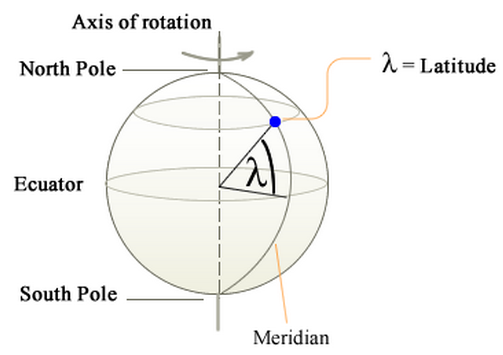
\includegraphics[scale=0.6]{Graphics/midterm1p2}
\end{center}

(a) a point on the Equator.''

Okay, first off, all of these problems will require the radius in meters, and the period in seconds, so let's start out by finding those two. The radius is then $\SI{6.38e6}{m}$, and the period $23 \cdot 3600 + 56 \cdot 60 + 4 = 86164$ seconds.

Next, let's find symbolic formulas for the two quantities they want. Both depend on the ``effective'' radius, which is the largest at the equator at $r = r_E$ and smallest at the poles, at $r = 0$ (at one single point). This radius depends on the angle from the equator, i.e. the latitude. The relationship can be derived with trigonometry, or essentially by guessing -- it is a trig function of the angle, such that the function is maximized at an angle of zero (from the equator), and minimized at 90 degrees... In other words, the cosine:

\begin{equation}
r = R_E \cos \lambda
\end{equation}

Not the most rigorous derivation, but I'm already completely sure that it's correct, so I won't really bother deriving it under an exam.

The velocity (or speed, rather) is found as

\begin{equation}
v = \frac{2 \pi r}{T} = \frac{2 \pi R_E \cos \lambda}{T}
\end{equation}

while the centripetal acceleration is found as

\begin{equation}
|a_c| = \frac{v^2}{r} = \frac{4 \pi^2 r^2}{r T^2} = \frac{4 \pi^2 r}{T^2} = \frac{4 \pi^2 R_E \cos \lambda}{T^2}
\end{equation}

As functions of $\lambda$ alone, we find

\begin{align}
v(\lambda) &= \frac{2 \pi (\SI{6.38e6}{m}) \cos \lambda}{\SI{86164}{s}}\\
|a_c(\lambda)| &= \frac{4 \pi^2 (\SI{6.38e6}{m}) \cos \lambda}{(\SI{86164}{s})^2}
\end{align}

Finally, we can simply plug in the numbers, and find, at the equator ($\lambda = 0$):

\begin{align}
v &= \SI{465.24}{m/s}\\
|a_c| &= \SI{0.0339}{m/s^2}
\end{align}

``(b) Zurich (latitude $\lambda = \ang{47.40}$ N).''

North or south doesn't matter, the radius ``tapers off' equally in both directions. We stick the numbers in, and find

\begin{align}
v &= \SI{314.908}{m/s}\\
a &= \SI{0.022963}{m/s^2}
\end{align}

``(c) Melbourne (latitude $\lambda = \ang{37.80}$ S).

\begin{align}
v &= \SI{367.61}{m/s}\\
a &= \SI{0.026807}{m/s^2}
\end{align}

``(d) the South Pole.''

Both are zero for $\lambda = \ang{90}$.

\section{Problem 3: Bucket in rotation}

``A bucket of water is swung in a vertical plane at the end of a rope of length $\ell$ = 3 m. The mass of the bucket plus water is 5 kg and the gravitational acceleration is $g = \SI{10}{m/s^2}$. We assume that the mass of the rope can be neglected.

(a) What is the minimal speed of the bucket at its highest point in the circular motion, such that the water does not fall out? (in m/s)''

The condition we need to meet is essentially $|a_c| > g$.

Since

\begin{equation}
|a_c| = \frac{v^2}{r}
\end{equation}

we can solve for $v$, and find

\begin{align}
v = \sqrt{r |a_c|}
\end{align}

Substitute in $r = \ell = \SI{3}{m}$ and $|a_c| = g = \SI{10}{m/s^2}$ and we find that

\begin{equation}
v = \sqrt{30} = \SI{5.477}{m/s}
\end{equation}

``(b) For this speed, what is the magnitude of the centripetal acceleration that the water in the bucket experiences at the highest point?''

The centripetal acceleration must cancel out gravity, so the answer is simply $g = \SI{10}{m/s^2}$.

``(c) At the lowest point,

(1) the speed is higher and the centripetal acceleration is lower than at the highest point of the circular motion.\\
(2) the speed is lower and the centripetal acceleration is higher than at the highest point of the circular motion.\\
(3) the speed is higher and the centripetal acceleration is higher than at the highest point of the circular motion.\\
(4) the speed is lower and the centripetal acceleration is lower than at the highest point of the circular motion.\\
(5) speed and centripetal acceleration are the same as at the highest point of the circular motion.''

This was the only (sub)question I missed on this exam, solely because I didn't interpret the question correctly and pretty much guessed at the answer. If we assume uniform circular motion, the speed and centripetal acceleration will be the same everywhere, but that interpretation doesn't make a whole lot of sense. It's incorrect, though.

A second interpretation is even worse: if we think of this as an extension of the previous two parts, we find

``What is the minimal speed of the bucket at its highest point in the circular motion, such that the water does not fall out?\\
At the lowest point: ...''

So it can be interpreted to be asking what the minimum speed and centripetal acceleration necessary is at the bottom, which doesn't make a lot of sense, either. This, too, will give the wrong answer.

Embarrassingly, I didn't quite get the question until after the exam. The \emph{intended} interpretation is that \emph{gravity is the only other force acting on the bucket}, so after it has fallen down \emph{due to gravity}, will the speed have increased or decreased? What about the centripetal acceleration?

Well, duh! All of a sudden I find this as easy as I expect most students did at once...\\
Gravity accelerates it downward, so clearly the speed must have increased after the ``fall''. The centripetal acceleration is proportional to $v^2$, so clearly that too must have increased.

\section{Problem 4: Elevator problem}

``An elevator is stopped at the ground floor. It starts moving upwards at constant acceleration $a > 0$ for 5 seconds. It then keeps a constant speed for 35 seconds. Finally, it slows down with an acceleration of the same magnitude (but opposite direction) $-a$, until it comes to a halt at the top floor. The top floor is 410 meters above the ground floor.

(a) What is the maximal speed v of the elevator ? (in m/s)\\
(b) What is the acceleration $a$? (in $\text{m/s}^2$)''

First, I will use a coordinate system where $y$ is positive upwards. I use $y$ instead of $x$ despite there being only one dimension, since I'm used to having $y$ upwards.

Okay, so there are three phases: constant acceleration at $a$ for 5 seconds, constant velocity for 35 seconds, and constant acceleration (or deceleration) at $-a$ for 5 seconds: since $a$ is the same in either case, it must come to a halt in the same time it took to accelerate up to that velocity in the first place.

For the first phase, we set $t = 0$ and $y_0 = 0$. We find the distance covered to be 

\begin{equation}
y_{acc} = \frac{1}{2} a t^2 = (\SI{12.5}{s^2}) a
\end{equation}

For the second, we know that the time taken is 35 seconds, and that the velocity must be given by $v = a t$, where $t = \SI{5}{s}$ (the time it spends to accelerate). We reset the clock, and find

\begin{equation}
y_{const} = v_0 t = (\SI{5}{s})a \cdot (\SI{35}{s}) = (\SI{175}{s^2}) a
\end{equation}

Finally, it comes to a halt; we again reset the clock, and use both $v_0$ (above) and $a$ here:

\begin{align}
y_{dec} &= (\SI{5}{s})a \cdot (\SI{5}{s}) - \frac{1}{2} a (\SI{5}{s})^2\\
       &= (\SI{25}{s^2}) - (\SI{12.5}{s^2}) a = (\SI{12.5}{s^2}) a
\end{align}

We add all of these displacements up:

\begin{align}
y_{total} &= (\SI{12.5}{s^2}) a + (\SI{175}{s^2}) a + (\SI{12.5}{s^2}) a\\
          &= (\SI{200}{s^2}) a
\end{align}

We know from the problem that this distance covered must equal $\SI{410}{m}$, so we set it equal to that and solve for $a$.

\begin{align}
(\SI{200}{s^2}) a &= \SI{410}{m}\\
a &= \frac{\SI{410}{m}}{\SI{200}{s^2}} = \SI{2.05}{m/s^2}
\end{align}

Does this answer make sense? Let's try it out. The distance covered during both the acceleration phases would be 51.25 meters, which leaves 358.75 meters for the constant velocity phase. That would require a constant velocity of 10.25 meters per second, which is indeed the velocity you would reach at \SI{2.05}{m/s^2} for 5 seconds. The answers are indeed marked as correct.

\section{Problem 5: Vertically thrown stones}

``A stone is thrown up vertically from the ground (the gravitational acceleration is $g = \SI{10}{m/s^2}$). After a time $\Delta t$ = 2 s, a second stone is thrown up vertically. The first stone has an initial speed $v_1 = \SI{18.0}{m/s}$, and the second stone $v_2 = \SI{18.0}{m/s}$.

(a) At what time t after the first stone is thrown will the two stones be at the same altitude h above ground? (in seconds)\\
(b) At what altitude h above ground will the two stones meet? (in meters)''

Let's set $y_0$ at the point they are thrown from, and $t = 0$ when the first is thrown. Therefore, the second is thrown at $t = \Delta t$, and we need to use $(t - \Delta t)$ in the kinematics equations for the second object for it to work out.

With all that in mind, the two position equations are

\begin{align}
y_1(t) &= v_1 t - \frac{1}{2} g t^2 &&= v_1 t - 5 t^2\\
y_2(t) &= v_2 (t - \Delta t) - \frac{1}{2} g (t - \Delta t)^2 &&= v_2 t - v_2 \Delta t - 5(t - \Delta t)^2
\end{align}

Sanity check: if $\Delta t$ is 2, and $t = 2$ as well, $y_2(t) = 0$ as it should be.

We can now set the two equal, substitute in some values, and find $t$:

\begin{align}
v_1 t - 5 t^2 &= v_2 t - v_2 \Delta t - 5(t - \Delta t)^2\\
18 t - 5 t^2 &= 18 t - (18)(2) - 5(t - 2)^2\\
- 5 t^2 &= - 36 - 5(t^2 - 4t + 4)\\
0 &= - 36 + 20t - 20\\
t &= \frac{56}{20} = \SI{2.8}{s}
\end{align}

I originally wrote these equations with units, and got an incredible mess, and an incorrect answer (I didn't have to submit it to realize it was wrong, either!), so I re-did it without units, and got a number that looked much more reasonable.

Part (b) should now be easy, at least. We know the time, and so we can use either kinematic equation (since they are at the same location). I choose the first one, of course, since it's less complex.

\begin{align}
h &= v_1 t - (\SI{5}{m/s^2}) t^2\\
h &= (\SI{18}{m/s}) (\SI{2.8}{s}) - (\SI{5}{m/s^2}) (\SI{2.8}{s})^2\\
h &= \SI{50.4}{m} - \SI{39.2}{m} = \SI{11.2}{m}
\end{align}

And we are done.

\section{Problem 6: Stone off a cliff}

``A person is standing on the edge of a cliff of height $h = 22$ m. She throws a stone of mass $m = 0.2$ kg vertically down with speed $v_0 = 11$ m/s (stone 1) and another stone of the same mass vertically up at the same speed (stone 2). The gravitational acceleration is $g = \SI{10}{m/s^2}$.

(a) What is the speed of stone 1 at the bottom of the cliff? (in m/s)\\
(b) What is the speed of stone 2 at the bottom of the cliff? (in m/s)\\
(c) What is the time of flight of stone 1 when it hits the bottom of the cliff? (in s)\\
(d) What is the time of flight of stone 2 when it hits the bottom of the cliff? (in s)\\
(e) What is the average speed of stone 1 during its flight? (in m/s)\\
(f) What is the average speed of stone 2 during its flight? (in m/s)\\
(g) What is the magnitude of the average velocity of stone 1 during its flight?\\
(h) What is the magnitude of the average velocity of stone 2 during its flight?''

Goodness! I might need the multiple tries just for typo correction with so many things to work out!

Since the stones are independent of each other, I will do a/c/e/g first, and b/d/f/h later.

We should know at this point that the mass is completely irrelevant for this problem, at least if we ignore air resistance.\\
Relevant kinematic equations for the first stone are, with $+y$ chosen upwards and $y = 0$ at the bottom of the cliff:

\begin{align}
y(t) = \SI{22}{m} - (\SI{11}{m/s}) t - \frac{1}{2} g t^2\\
v(t) = - \SI{11}{m/s} - g t
\end{align}

We first need to know the time $t$ when it hits the ground. We can find it from the first equation, set equal to 0.

\begin{align}
0 &= \SI{22}{m} - (\SI{11}{m/s}) t - \frac{1}{2} (\SI{10}{m/s^2}) t^2\\
0 &= (\SI{5}{m/s^2}) t^2 + (\SI{11}{m/s}) t - \SI{22}{m}
\end{align}

Besides the units, this is just a simple quadratic equation, with the solution 

\begin{equation}
t = \frac{-11 \pm \sqrt{11^2 - 4\cdot5\cdot(-22)}}{10} = -1.1 \pm 2.3685 = \SI{1.2685}{s}
\end{equation}

... if we neglect the negative solution, as we should! That answers (c), then. Now, back to (a), the speed.

\begin{equation}
v(t) = \Big|- \SI{11}{m/s} - (\SI{10}{m/s^2})(\SI{1.2685}{s})\Big| = \SI{23.685}{m/s}
\end{equation}

``(e) What is the average speed of stone 1 during its flight? (in m/s)''

Average speed is simply distance divided by time. It travels $h$ meters in $t$ seconds, so we find

\begin{equation}
\overbar{v}_1 = \frac{h}{t} = \frac{\SI{22}{m}}{\SI{1.2685}{s}} \approx \SI{17.343}{m/s}
\end{equation}

``(g) What is the magnitude of the average velocity of stone 1 during its flight?''

Because it has traveled in one direction only, the distance is equal to the displacement, and so the magnitude of the average velocity is equal to the average speed.

Next up: the second stone. I will simply solve this as a separate problem, instead of relating the two. Since the workings will be about the same as above, I'll keep in briefer, though.

\begin{align}
y(t) = \SI{22}{m} + (\SI{11}{m/s}) t - \frac{1}{2} g t^2\\
v(t) = \SI{11}{m/s} - g t
\end{align}

Note that the initial velocity is now upwards. We again solve for the time, and find $t = \SI{3.46854}{s}$ to hit the bottom, which answers (d). Plugging that into $v(t)$, we find the speed as it hits, which answers (b): $|v(3.46854)| = \SI{23.685}{m/s}$. Same as the other one -- I suspected as much, but in the interest of avoiding silly mistakes, I chose to solve them separately anyhow.

Next, average speed. This one differs: we now have the upwards movement PLUS the downwards movement, divided by the time.\\
How far above the throw point did it reach? With the launch velocity, it must have reached the top at $t = \SI{1.1}{s}$, which translates into reaching 6.05 meters up. It then falls back down 6.05 meters, plus the 22 meters below the starting point, for a total of 34.1 meters, divided by the time:

\begin{equation}
\overbar{v}_2 = \frac{\SI{34.1}{m}}{\SI{3.46854}{s}} = \SI{9.83}{m/s}
\end{equation}

And, finally, magnitude of the average velocity. Here, only displacement matters, and it ends up 22 meters below where it started:

\begin{equation}
\widetilde{v}_2 = \frac{\SI{22}{m}}{\SI{3.46854}{s}} = \SI{6.34}{m/s}
\end{equation}

\section{Problem 7: Stone on roof, find distance}

\begin{center}
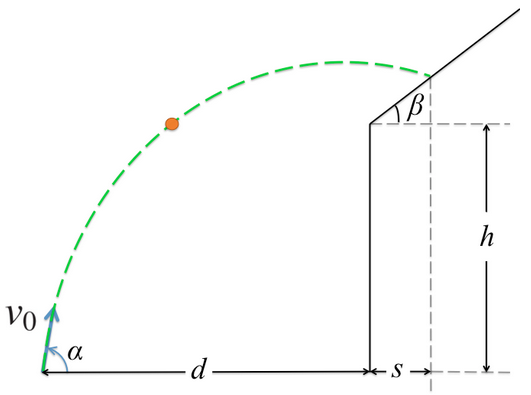
\includegraphics[scale=0.6]{Graphics/midterm1p7}
\end{center}

``We are standing at a distance $d = 15$ m away from a house. The house wall is $h = 6$ m high and the roof has an inclination angle $\beta = \ang{30}$. We throw a stone with initial speed $v_0 = \SI{20}{m/s}$ at an angle $\alpha = \ang{51}$. The gravitational acceleration is $g  =\SI{10}{m/s^2}$. (See figure)

(a) At what horizontal distance from the house wall is the stone going to hit the roof ($s$ in the figure)? (in meters)\\
(b) What time does it take the stone to reach the roof? (in seconds)''

This problem is scaring me a bit: there have been \emph{many} reports on the wiki from students who claim it's failing their correct answers. The staff insist that all such answers are incorrect, though. So the question is: when (or if) I think I've solved it, will I have made the same mistake they all did, or will I have \emph{actually} solved it? I suppose there's only one way to find out...

Among the staff hints are

\begin{itemize}
\item Make sure you use $g = \SI{10}{m/s^2}$
\item Make sure you don't round answers to less than 2-3 decimals
\item Solve (a) independently from (b).
\item Make sure you are not making any uncalled for approximations.
\item Do not waste attempts by plugging the value of $d+s$, or simply rounding your answer.
\end{itemize}

Okay, let's see. I will begin by writing down the kinematics equations, and we'll see where that gets us. This is of course the easy part. I choose a coordinate system centered at the throw, with $+\hat{x}$ to the right and $+\hat{y}$ upwards.

\begin{align}
x(t)   &= (v_0 \cos \alpha) t\\
v_x(t) &= v_0 \cos \alpha\\
y(t)   &= (v_0 \sin \alpha) t - \frac{1}{2} g t^2\\
v_y(t) &= v_0 \sin \alpha - g t
\end{align}

Both the $x$ and $y$ position of where it hits the roof depend on $\beta$. If $\beta = 0$, clearly it will hit at $y = h$, and with a large value of $s$. If $\beta = \ang{90}$, the ``roof'' is more like a wall, and it hits at $x = d$, with $s = 0$. In between these extremes, $x > d$ (so $s > 0$) and $y > h$.

I'm not really sure how to solve this, but one way that may work is to try to find the roof height (above $h$) as a function of $x$ beyond the house edge, where it starts. Clearly, it should be $0$ just at the house edge, and go toward infinity for ridiculously high values of $x$ (since it has no defined end, it just keeps going in the direction shown in the figure).

If we draw just a simple triangle as the ``roof'', and mark out $\beta$, and a point along the hypotenuse we call $(x, y)$, we find that

\begin{align}
\tan \beta &= \frac{y}{x}\\
y &= x \tan \beta
\end{align}

This makes sense -- if $\beta = \ang{45}$, $y = x$, i.e. they increase at the same rate as you go towards the right. If $\beta$ is really large, $y$ grows very fast as $x$ grows a little, and if $\beta$ is very low, $y$ barely grows at all as you go further to the right.

What I just called $x$ is really the same as $s$ in the problem, so I will use that from now on. The $y$ coordinate where it hits, as measured with $x = 0$ and $y = 0$ centered on the throw, is then $y = h + s \tan \beta$ and $x = d + s$. I'm not sure what the staff meant by not ``wast[ing] attempts by plugging the value of $d+s$'', but I don't see how that could be incorrect, so I will try this out.

Using the kinematics equations, we then have

\begin{align}
(v_0 \cos \alpha) t &= d + s\\
(v_0 \sin \alpha) t - \frac{1}{2} g t^2 &= h + s \tan \beta
\end{align}

The unknowns are $t$ and $s$, and those are exactly the values the problem asks for us to find. Awesome!

Since it is allowed, I solved these equations in Mathematica, and found $s = \SI{9.301730802}{m}$ and $t = \SI{1.930791624}{s}$. Ridiculous precision, but since so many students had trouble with it, I decided to submit with all those decimals instead of possibly rounding too much.

I figured I would also solve the equations manually, but honestly, it turned out to be a bit too bad, at least with the first method I tried (solve first equation for $t$, substitute into second, solve for $s$). Tons of terms, $\tan \alpha$ and $\cos \alpha$ everywhere, $s$ in 3-4 different terms, some inside squared expressions that you'd have to multiply out, etc, etc.

The staff solution does this better by using $x - d$ instead of $s$, which simplifies things a bit. The full answer is still not pretty, though. This is what Mathematica gives me, fully simplified taking into account things such as $g > 0$, $0 < \alpha < \pi/2$ etc.:

\begin{equation}
s = \frac{v_0 \cos (\alpha) \left(\sqrt{2 d g \tan (\beta) - 2 g h + v_0^2 \sec ^2(\beta) \sin^2(\alpha -\beta)} + v_0 \sec (\beta) \sin (\alpha - \beta)\right) - d g}{g}
\end{equation}

\begin{equation}
t = \frac{\sqrt{2 d g \tan (\beta) - 2 g h + v_0^2 \sec^2(\beta) \sin^2(\alpha - \beta)} + v_0 \sec(\beta) \sin (\alpha - \beta)}{g}
\end{equation}

Wow.

\section{Problem 8: Man on a flatcar with ball}

\begin{center}
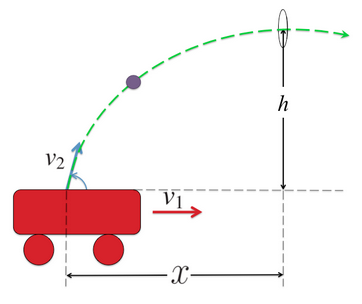
\includegraphics[scale=0.6]{Graphics/midterm1p8}
\end{center}

``A person is riding on a flatcar traveling at a constant speed $v_1 = \SI{15}{m/s}$ with respect to the ground. He wishes to throw a ball through a stationary hoop in such a manner that the ball will move horizontally as it passes through the hoop. The hoop is at a height $h = \SI{4}{m}$ above his hand. He throws the ball with a speed $v_2 = \SI{14}{m/s}$ with respect to the flatcar. Let $g = \SI{10}{m/s^2}$ and neglect air drag completely. (see figure)

(a) At what horizontal distance $x$ in front of the hoop must the person release the ball? (in meters)\\
(b) When the ball leaves his hand, what is the direction of the velocity vector of the ball as seen from the flatcar? (angle $\alpha_{car}$ with respect to the horizontal in degrees)\\
(c) When the ball leaves his hand, what is the direction of the velocity vector of the ball as seen from the ground? (angle $\alpha_{ground}$ with respect to the horizontal in degrees)''

I'll try to do most of the work in a coordinate system fixed to the ground, such that the flatcar is moving forward at $v_1$.

So, from this frame, at what velocity is the ball thrown? The car moves horizontally forward, so clearly the $y$ component (which I choose to be positive upwards) will not change. Instead, using prime notation for the launch velocity as seen from the ground,

\begin{align}
v_2' = (v_2 \cos \alpha_{car} + v_1) \hat{x} + (v_2 \sin \alpha_{car}) \hat{y}
\end{align}

A bit of a cumbersome way to write it, but the point is that only the $x$ component will change.

Writing these as components, then, we we of course have

\begin{align}
v_{2x}' &= v_2 \cos \alpha_{car} + v_1\\
v_{2y}' &= v_2 \sin \alpha_{car}
\end{align}

We can now calculate the distance $x$ as if we were standing still on the ground and throwing the ball, instead, with less of a headache... at least hopefully.\\
The condition is that it must move horizontally through the hoop. Since it moves in a parabola, this means (as is evident from the drawing, too) that it must be at its apex when it moves through. That happens when $v_{2y} = 0$, for one.

In fact, we can ignore $x$ motion almost completely, unless I'm missing something! We find when $v_{2y} = 0$, and extract the time from that equation. Unfortunately, the angle is also unknown. We can find it by also relating the $y$ \emph{position} to the height $h$, though.\\
Anyway, let's set up the kinematics equations. I will write them from the reference frame fixed to the ground. $x_0 = 0$ is where the ball is launched, which is $x$ meters in front of the hoop.

\begin{align}
x(t)   &= (v_1  + v_2 \cos \alpha_{car}) t\\
v_x(t) &= v_1 + v_2 \cos \alpha_{car}\\
y(t)   &= (v_2 \sin \alpha_{car}) t - \frac{1}{2} g t^2\\
v_y(t) &= v_2 \sin \alpha_{car} - g t
\end{align}

So at some value for $t$, we should have $y(t) = h$ and $v_y(t) = 0$. The equations have $\alpha_{car}$ and $t$ as unknowns, then, so this should be solvable. Let's do it. Let's solve the simple one for $\alpha_{car}$:

\begin{align}
v_2 \sin \alpha_{car} - g t = 0\\
\sin \alpha_{car} = \frac{g t}{v_2}\\
\alpha_{car} = \arcsin \frac{g t}{v_2}
\end{align}

Next, we need to find an expression for $t$:

\begin{align}
h = (v_2 \sin \alpha_{car}) t - \frac{1}{2} g t^2\\
(2 v_2 \sin \alpha_{car}) t - g t^2 = 2h\\
g t^2 - (2 v_2 \sin \alpha_{car}) t = -2h
\end{align}

Before we move on, we can substitute in the angle. We get the sine of the arcsine, so we end up without trig functions:

\begin{align}
g t^2 - (2 v_2 \frac{g t}{v_2}) t = -2h\\
g t^2 - (2 g t) t = -2h\\
-g t^2 = -2h\\
t = \sqrt{\frac{2h}{g}} \approx \SI{0.8944}{s}
\end{align}

We can now find $\alpha_{car}$ using the expression we had above:

\begin{equation}
\alpha_{car} = \arcsin \frac{g t}{v_2} \approx 0.693012 \text{ rad} \approx \ang{39.707}
\end{equation}

Nice. We now have what we need to find $x$, since we have a kinematic equation for it:

\begin{equation}
x = (v_1  + v_2 \cos \alpha_{car}) t = (\SI{15}{m/s} + (\SI{14}{m/s}) \cos(\ang{39.707})) (\SI{0.8944}{s}) = \SI{23.049}{m}
\end{equation}

Finally, we need to find the angle as seen from the ground. Intuitively, how would the angle change? I think it should become less steep, i.e. a smaller angle. If we imagine the car moving really, really fast (to be silly, say 10 km/s), so that $v_1 \gg v_2$, the throw is almost exclusively in the $x$ direction as seen from the ground; he might throw it upwards at 10-20 m/s and forward at 10-20 m/s, but with the 10 \emph{km} per second relative movement, his throw really doesn't matter. The angle must be very, very small in that case. 

Now, how do we calculate it? The easiest way I can think of is to calculate the velocity vector (as seen from the ground), and then do some basic trigonometry. We have the four kinematics equations above; at $t = 0$, their values are

\begin{align}
v_x(0) = v_1 + v_2 \cos \alpha_{car} = \SI{15}{m/s} + (\SI{14}{m/s}) \cos(\ang{39.707}) = \SI{25.77}{m/s}\\
v_y(0) = v_2 \sin \alpha_{car} = (\SI{14}{m/s}) \sin(\ang{39.707}) = \SI{8.944}{m/s}
\end{align}

The angle can then be found by drawing this up and realizing that we need the arctangent of $v_y$ over $v_x$:

\begin{align}
\alpha_{ground} = \arctan \frac{v_y}{v_x} \approx \ang{19.140}
\end{align}

Indeed, if $v_x$ grows, the angle gets smaller, as predicted.\\
That's it for this exam!

\end{document}